% ==============================================================================
% PAGE 36: CHAPTER-5 CONSTRUCTION - PART 1 (Numbered Page 28)
% ==============================================================================
\begin{center}
  {\fontsize{15}{18}\selectfont \bfseries \textcolor{red!80!black}{\underline{CHAPTER-5}}}\\[2mm]
  {\fontsize{16}{20}\selectfont \bfseries \textcolor{red!80!black}{\underline{CONSTRUCTION}}}\\[4mm]
  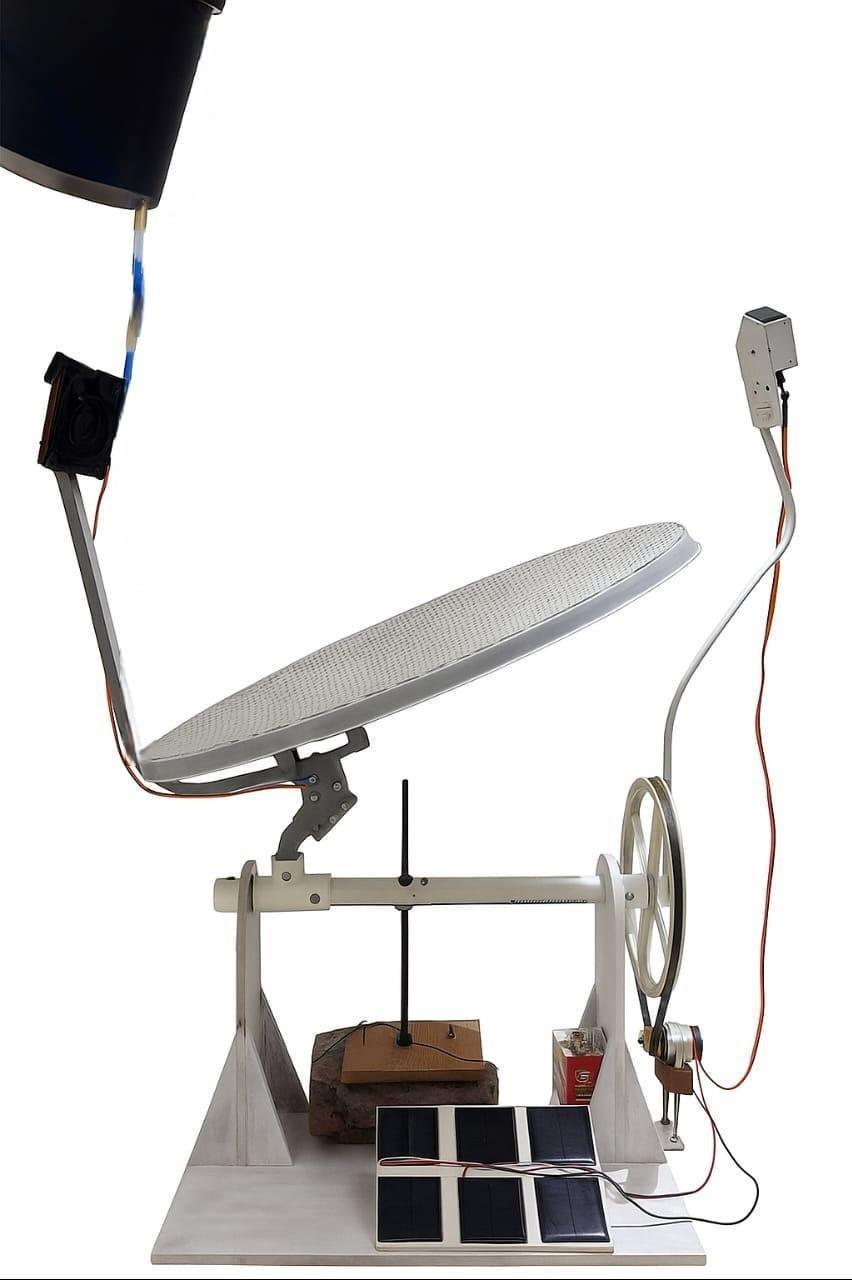
\includegraphics[width=90mm]{figures/fig16_actual_model.jpg}\\[5mm]
\end{center}

\noindent
\begin{spacing}{1.2}
{\fontsize{10.2}{14.5}\selectfont
The construction of the Parabolic Solar Water Heater with Automatic Tracking and Power Generation begins with preparing a strong base structure. A wooden sheet of $60\text{ cm} \times 60\text{ cm}$ is used as the base platform to support all components. A PVC pipe shaft is mounted horizontally at the center of this base to act as the main support for the parabolic dish. The end caps are fitted at the end of the shaft to allow smooth rotational movement. The base and supporting parts are properly aligned, drilled, and painted with white colour to prevent damage of electronic components from sunlight. All joints are fixed using nuts, bolts, and adhesive for proper strength and balance.
}
\end{spacing}
\clearpage
